\chapter{Distance propre, géométrie de Kruskal et observateurs de l’horizon}

La métrique de Schwarzschild semble devenir singulière à l’horizon. La courbure, elle, ne l’est pas. Pour distinguer ces deux affirmations, nous éliminons d’abord l’échelle globale du trou noir, puis remplaçons la coordonnée radiale par la distance propre à l’horizon. Au voisinage de celui-ci, la géométrie obtenue est celle d’un espace-temps plat ordinaire décrit en coordonnées accélérées. Une fois cette géométrie représentée, les questions concernant Alice, Bob et Charlie portent sur les lignes d’univers et les rayons lumineux, plutôt que sur des paradoxes verbaux.

\section{Éliminer le rayon de Schwarzschild par changement d’échelle}

Commençons par des coordonnées primées, afin que les variables redimensionnées puissent ensuite recevoir les noms usuels :
\begin{equation}
d\tau^2
=
\left(1-\frac{2MG}{r'}\right)dt'^2
-
\frac{dr'^2}{1-\frac{2MG}{r'}}
-
r'^2d\Omega_2^2.
\label{eq:l7-schwarzschild-dimensional}
\end{equation}
Introduisons le rayon de Schwarzschild et les coordonnées sans dimension
\begin{equation}
r_{\mathrm S}=2MG,
\qquad
r=\frac{r'}{r_{\mathrm S}},
\qquad
t=\frac{t'}{r_{\mathrm S}}.
\label{eq:l7-rescaling}
\end{equation}
Nous posons \(c=1\), de sorte que le temps et la longueur ont la même unité. Le rayon \(r_{\mathrm S}\) est donc à la fois une longueur et le temps de parcours de la lumière correspondant à cette longueur. La substitution donne
\begin{equation}
d\tau^2
=r_{\mathrm S}^2
\left[
\left(1-\frac1r\right)dt^2
-
\frac{dr^2}{1-\frac1r}
-
r^2d\Omega_2^2
\right].
\label{eq:l7-schwarzschild-rescaled}
\end{equation}
Tous les trous noirs de Schwarzschild non rotatifs et non chargés ont donc la même géométrie sans dimension. La variation de la masse change le facteur d’échelle qui multiplie la métrique, mais pas la forme de l’expression entre crochets. C’est comme si l’on dessinait des sphères après avoir divisé toutes les distances par leur rayon : le même dessin représente la Lune et la Terre, même si un centimètre sur chaque dessin correspond à une distance physique différente.

\begin{classroomqa}
\audiencequestion{Quels signes accompagnent les termes radial et angulaire de la métrique ?}
\lecturerresponse{Avec la signature \(+---\) utilisée ici, les deux termes spatiaux portent un signe moins. La salle a repéré le signe pendant que l’expression était écrite. Le facteur angulaire peut comporter un sinus ou un cosinus selon que la coordonnée polaire est mesurée depuis l’axe ou depuis l’équateur ; la notation compacte \(d\Omega_2^2\) évite cette question de convention.
\lecturetimestamp{00:07:48--00:08:12}}
\end{classroomqa}

\section{L’échelle de courbure à l’horizon}

Le changement d’échelle permet de répondre à une importante question physique sans long calcul tensoriel. Une composante de la métrique est sans dimension. Un symbole de Christoffel contient une dérivée par rapport à une coordonnée et a donc les dimensions de l’inverse d’une longueur, tandis qu’une composante du tenseur de Riemann dans un repère orthonormé physique a les dimensions
\begin{equation}
[g_{\mu\nu}]=1,
\qquad
[\Gamma^\mu{}_{\nu\rho}]=L^{-1},
\qquad
[R_{\hat\alpha\hat\beta\hat\gamma\hat\delta}]
=L^{-2}.
\label{eq:l7-curvature-dimensions}
\end{equation}
À l’horizon \(r=1\), la seule longueur physique disponible est \(r_{\mathrm S}\). L’échelle de la courbure de marée doit donc être
\begin{equation}
\left|R_{\hat\alpha\hat\beta\hat\gamma\hat\delta}\right|_{\mathrm{hor}}
\sim \frac{1}{r_{\mathrm S}^2}.
\label{eq:l7-horizon-curvature}
\end{equation}
Plus généralement, elle est égale à \(r_{\mathrm S}^{-2}\) fois une fonction sans dimension de \(r\). Cette affirmation concerne le champ de marée de Riemann, et non le scalaire de Ricci, qui s’annule dans le vide de Schwarzschild.

La conclusion physique est immédiate. Quand la masse augmente, \(r_{\mathrm S}\) augmente et le champ de marée à l’horizon s’affaiblit. Un petit trou noir peut déchirer un corps étendu pendant sa traversée ; près de l’horizon d’un trou noir supermassif, les forces de marée peuvent être faibles. La courbure augmente néanmoins vers l’intérieur et diverge en \(r=0\). L’horizon et la singularité sont donc des objets radicalement différents.

\section{Distance propre à l’horizon}

Pour la suite du calcul local, posons \(r_{\mathrm S}=1\). En relativité, les changements de coordonnées ne sont pas une simple question d’apparence : de mauvaises coordonnées peuvent dissimuler une géométrie régulière derrière des coefficients singuliers. La différence de coordonnées de Schwarzschild \(r-1\) n’est pas la distance radiale mesurée depuis l’horizon.

\begin{figure}[htbp]
\centering
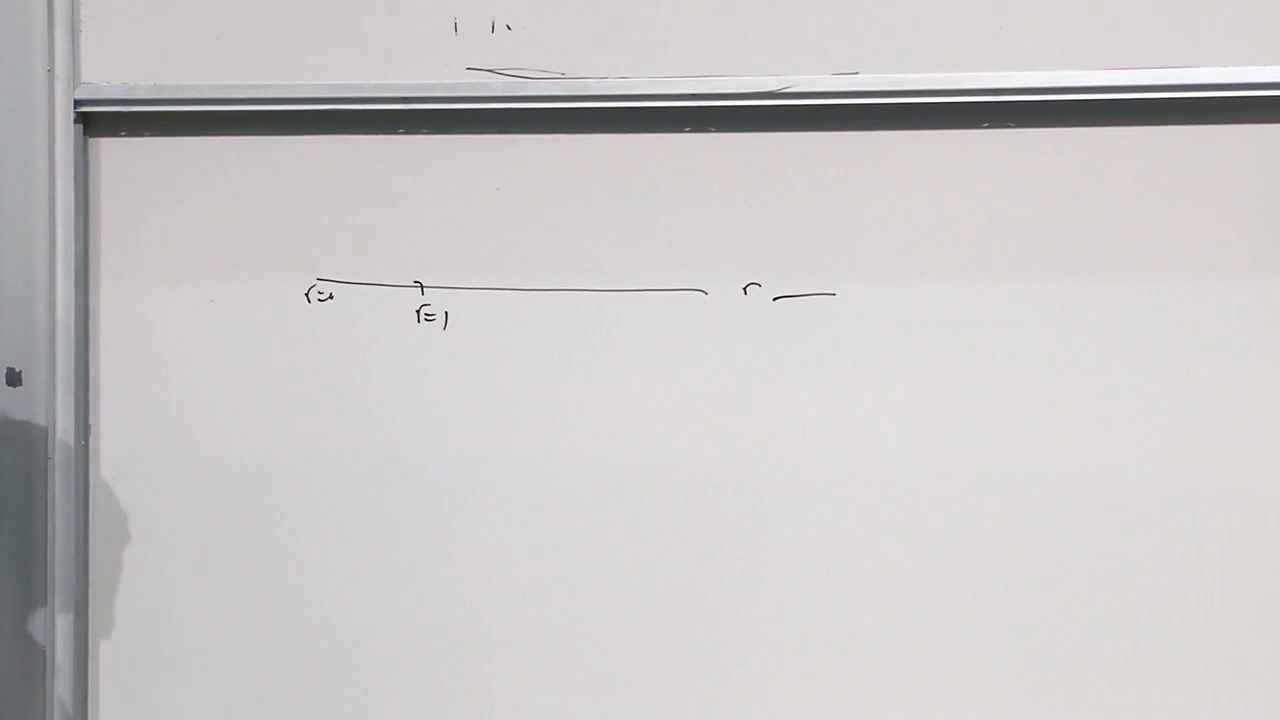
\includegraphics[width=0.78\textwidth]{lecture_07_figure_02.png}
\caption{La ligne de coordonnée radiale tracée au tableau. L’horizon se trouve en \(r=1\), tandis que \(r=0\) est la singularité de courbure.}
\lectureframe{00:16:11}
\end{figure}

Fixons \(t\) et les angles. L’élément de longueur spatiale positif est alors
\begin{equation}
ds^2=\frac{dr^2}{1-\frac1r},
\qquad
ds=\sqrt{\frac{r}{r-1}}\,dr.
\label{eq:l7-radial-proper-line}
\end{equation}
Définissons la distance propre sans dimension à l’horizon par
\begin{equation}
\rho(r)
=
\int_1^r\sqrt{\frac{r'}{r'-1}}\,dr'.
\label{eq:l7-rho-definition}
\end{equation}
Lorsque l’échelle globale est rétablie, la distance physique vaut \(r_{\mathrm S}\rho\). Nous n’aurons pas besoin de la forme explicite de l’intégrale. Seule sa dérivée nous importe :
\begin{equation}
\frac{d\rho}{dr}
=\sqrt{\frac{r}{r-1}},
\qquad
d\rho^2
=\frac{dr^2}{1-\frac1r}.
\label{eq:l7-rho-derivative}
\end{equation}
Le terme radial compliqué devient donc exactement \(-d\rho^2\). C’est pour cette simplification que nous introduisons \(\rho\).

Redimensionnons maintenant une nouvelle fois la coordonnée temporelle :
\begin{equation}
\omega=\frac{t}{2}.
\label{eq:l7-omega}
\end{equation}
Comme \(r\) est une fonction de \(\rho\), la métrique peut s’écrire
\begin{equation}
d\tau^2
=
F(\rho)\rho^2d\omega^2
-
d\rho^2
-
r(\rho)^2d\Omega_2^2.
\label{eq:l7-rho-metric}
\end{equation}

\begin{classroomqa}
\audiencequestion{La définition de \(F(\rho)\) vise-t-elle simplement à donner au coefficient temporel la forme \(F(\rho)\rho^2\) ?}
\lecturerresponse{Oui. À ce stade, cette factorisation n’a pas de contenu physique indépendant. C’est une définition commode. Son utilité apparaît lorsqu’on considère les limites de \(F\) près de l’horizon et loin de celui-ci.
\lecturetimestamp{00:26:39--00:26:59}}
\end{classroomqa}

Loin du trou noir, le coefficient temporel de Schwarzschild tend vers un. Comme \(dt=2d\omega\), on obtient
\begin{equation}
\lim_{\rho\to\infty}F(\rho)\rho^2=4.
\label{eq:l7-far-limit}
\end{equation}
Près de l’horizon, l’équation~\eqref{eq:l7-rho-definition} donne
\begin{equation}
\begin{aligned}
\rho&\simeq 2\sqrt{r-1},\\
r(\rho)&=1+\frac{\rho^2}{4}+O(\rho^4),\\
\lim_{\rho\to0}F(\rho)&=1.
\end{aligned}
\label{eq:l7-near-expansion}
\end{equation}

\begin{figure}[htbp]
\centering
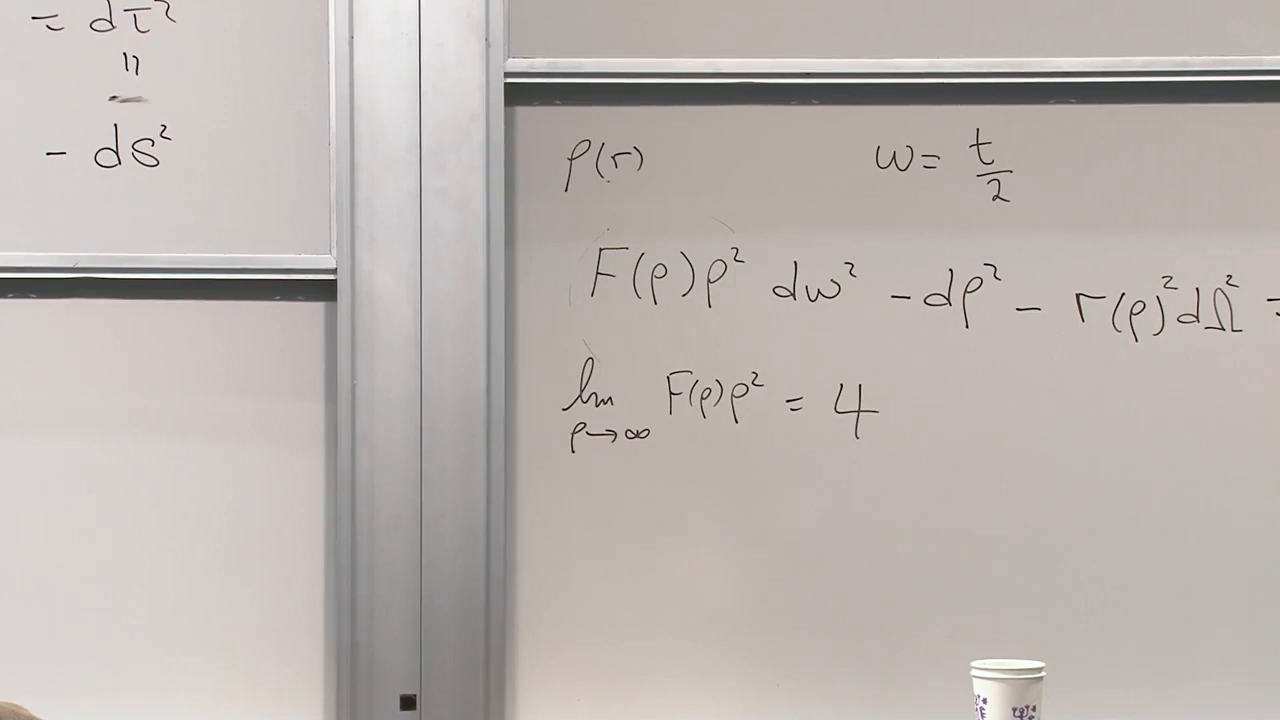
\includegraphics[width=0.90\textwidth]{lecture_07_figure_03.png}
\caption{La métrique en \((\rho,\omega)\), son coefficient temporel asymptotique et les limites près de l’horizon \(F\to1\) et \(r=1+\rho^2/4+\cdots\).}
\lectureframe{00:37:30}
\end{figure}

\section{L’espace-temps plat caché à l’horizon}

Au voisinage de \(\rho=0\), la partie radiale et temporelle de l’équation~\eqref{eq:l7-rho-metric} se réduit à
\begin{equation}
d\tau_{\mathrm{radial}}^2
\simeq
\rho^2d\omega^2-d\rho^2.
\label{eq:l7-rindler-metric}
\end{equation}
Il s’agit de l’espace-temps plat de Minkowski en coordonnées polaires hyperboliques. Définissons
\begin{equation}
X=\rho\cosh\omega,
\qquad
T=\rho\sinh\omega.
\label{eq:l7-rindler-transform}
\end{equation}
On obtient alors
\begin{equation}
dT^2-dX^2
=
\rho^2d\omega^2-d\rho^2.
\label{eq:l7-minkowski-check}
\end{equation}
Les courbes où \(\rho\) est constant vérifient
\begin{equation}
X^2-T^2=\rho^2
\label{eq:l7-constant-rho}
\end{equation}
ce sont des hyperboles. Les courbes où \(\omega\) est constant sont des demi-droites issues de l’origine. Lorsque \(\omega\to\infty\), ces demi-droites s’approchent de la droite nulle \(T=X\). L’horizon de Schwarzschild, qui semblait rejeté à un temps coordonné infini, est donc une droite nulle ordinaire dans le diagramme régulier.

\begin{figure}[htbp]
\centering
\includegraphics[width=0.88\textwidth]{lecture_07_figure_06.png}
\caption{La géométrie complète du tableau : hyperboles à \(\rho\) constant, demi-droites à \(\omega\) constant, horizon nul et région \(r<1\) au-dessus de celui-ci.}
\lectureframe{00:38:30}
\end{figure}

\begin{figure}[htbp]
\centering
\resizebox{0.96\linewidth}{!}{%
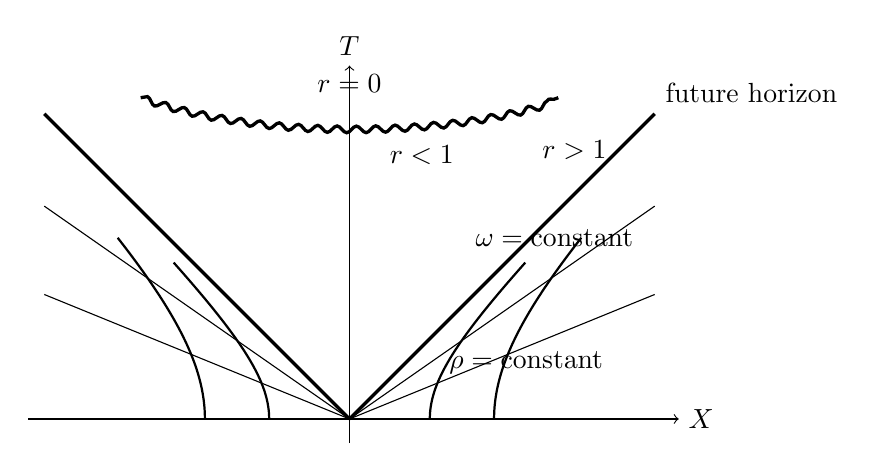
\begin{tikzpicture}[scale=1.02]
\draw[->] (-4.0,0) -- (4.1,0) node[right] {$X$};
\draw[->] (0,-0.3) -- (0,4.4) node[above] {$T$};
\draw[very thick] (0,0) -- (3.8,3.8)
  node[above right] {future horizon};
\draw[very thick] (0,0) -- (-3.8,3.8);
\draw[thick]
  plot[domain=0:1.42,samples=50]
  ({1.0*cosh(\x)},{1.0*sinh(\x)});
\draw[thick]
  plot[domain=0:1.05,samples=50]
  ({1.8*cosh(\x)},{1.8*sinh(\x)});
\draw[thick]
  plot[domain=0:1.42,samples=50]
  ({-1.0*cosh(\x)},{1.0*sinh(\x)});
\draw[thick]
  plot[domain=0:1.05,samples=50]
  ({-1.8*cosh(\x)},{1.8*sinh(\x)});
\draw[thin] (0,0) -- (3.8,1.55);
\draw[thin] (0,0) -- (3.8,2.65);
\draw[thin] (0,0) -- (-3.8,1.55);
\draw[thin] (0,0) -- (-3.8,2.65);
\draw[very thick,decorate,decoration={snake,amplitude=1.2pt,segment length=7pt}]
  (-2.6,4.0) .. controls (-1.2,3.5) and (1.2,3.5) .. (2.6,4.0);
\node at (0,4.18) {$r=0$};
\node at (2.2,0.7) {$\rho=\mathrm{constant}$};
\node at (2.55,2.25) {$\omega=\mathrm{constant}$};
\node at (0.9,3.28) {$r<1$};
\node at (2.8,3.35) {$r>1$};
\end{tikzpicture}
}
\caption{Une reconstruction causale nette. L’horizon est une droite nulle, tandis que la singularité de courbure \(r=0\) est une frontière future à l’intérieur du trou noir.}
\label{fig:l7-kruskal-clean}
\end{figure}

La limite où \(\rho\) devient petit diffère de la limite de petit rayon en coordonnées polaires euclidiennes. Un petit cercle euclidien se contracte vers un point. Une hyperbole à \(\rho\) constant s’approche d’une droite nulle entière. Ainsi, \(\rho=0\) désigne tout l’horizon, et pas seulement le point où les axes se croisent.

La formule extérieure peut être prolongée analytiquement jusqu’à \(r<1\). Près de l’horizon, \(r-1\simeq\rho^2/4\), de sorte que l’intérieur correspond formellement à \(\rho^2<0\). On peut qualifier \(\rho\) d’imaginaire, mais il est plus simple d’utiliser \(\rho^2\), \(r\) ou les coordonnées régulières \(T,X\). Les signes des coefficients de Schwarzschild associés à \(t\) et \(r\) s’échangent à l’intérieur. Cela ne signifie pas que la montre-bracelet physique se transforme en règle. Cela signifie que les coordonnées de Schwarzschild ont échangé leur caractère causal.

\begin{classroomqa}
\audiencequestion{Que représentent les hyperboles horizontales à l’intérieur de l’horizon, et que représentent les demi-droites ?}
\lecturerresponse{Les courbes hyperboliques correspondent à \(r\) constant, ou, de manière équivalente, à \(\rho^2\) constant, prolongé dans \(r<1\). Les demi-droites correspondent à un temps de Schwarzschild constant. À l’extérieur, elles forment un quadrillage commode pour les coordonnées ; à l’intérieur, il ne faut pas confondre ces mêmes étiquettes avec les trajectoires d’observateurs physiques.
\lecturetimestamp{00:44:12--00:44:59}}
\end{classroomqa}

\begin{classroomqa}
\audiencequestion{La direction verticale est-elle une coordonnée temporelle, et à quel référentiel correspond-elle ?}
\lecturerresponse{C’est une direction temporelle régulière dans le nouveau diagramme d’espace-temps, mais ce n’est pas le temps de Schwarzschild singulier \(t\). Le diagramme est adapté à la structure causale de la chute libre. Un observateur maintenu à rayon extérieur constant suit une hyperbole et doit accélérer ; un observateur en chute libre traverse l’horizon nul sans heurt.
\lecturetimestamp{00:45:54--00:46:48}}
\end{classroomqa}

\begin{classroomqa}
\audiencequestion{Si \(\rho^2<0\) à l’intérieur, où se trouve le facteur explicite \(i\) ?}
\lecturerresponse{On peut introduire un \(\rho\) imaginaire, mais cela n’apporte rien. Le contenu invariant est porté par \(r\), par \(\rho^2\) et par les coordonnées réelles et régulières \(T,X\). La relation \(r-1\simeq\rho^2/4\) n’est que le développement au voisinage de l’horizon.
\lecturetimestamp{00:52:35--00:53:00}}
\end{classroomqa}

Dans le cours, le diagramme régulier est souvent appelé diagramme de Kruskal. À proprement parler, les coordonnées exactes de Kruskal comprennent un facteur radial qui rend régulière la métrique de Schwarzschild complète, tandis que l’équation~\eqref{eq:l7-rindler-transform} en est la forme au voisinage de l’horizon. Le message causal reste le même : l’horizon est régulier, mais toute courbe future de genre temps ou nulle à l’intérieur se termine en \(r=0\). Aucun virage supraluminique ne peut la ramener à travers l’horizon.

\subsection{Comment la singularité de coordonnées a été comprise}

La régularité de l’horizon a longtemps été difficile à discerner, car les coordonnées originales de Schwarzschild donnent à ses coefficients une apparence singulière. Eddington, puis Finkelstein, ont introduit des coordonnées qui traversent l’horizon, et Finkelstein a reconnu la frontière causale à sens unique. Kruskal, qui maîtrisait les changements de coordonnées grâce à la physique des plasmas, a fourni une représentation globale régulière de la solution éternelle.

Le cours s’interrompt ensuite pour évoquer John Wheeler, qui a contribué à imposer l’expression « trou noir ». Cette pause est aussi personnelle qu’historique : Wheeler est resté dans les mémoires comme un ami doux et réfléchi, même si les jugements politiques, notamment sur la compétition nucléaire, divergeaient fortement. Une anecdote personnelle humoristique est racontée pour éviter de réduire Wheeler à une figure socialement conventionnelle. Le propos technique reprend avec la réplique : « les trous noirs n’ont pas de cheveux ». Un trou non rotatif perturbé retrouve rapidement une symétrie sphérique ; un trou en rotation évolue vers la forme stationnaire déterminée par ses paramètres conservés. C’est la version qualitative, dans ce cours, de l’idée d’absence de cheveux, et non une démonstration du théorème complet.

\section{Alice traverse l’horizon ; Bob reste à l’extérieur}

Le diagramme maximalement prolongé contient des régions qui n’existent pas dans l’espace-temps simple d’une étoile s’effondrant à partir de données initiales ordinaires. Pour l’expérience avec les observateurs, nous n’utilisons que l’extérieur, l’horizon futur et l’intérieur du trou noir.

\begin{figure}[htbp]
\centering
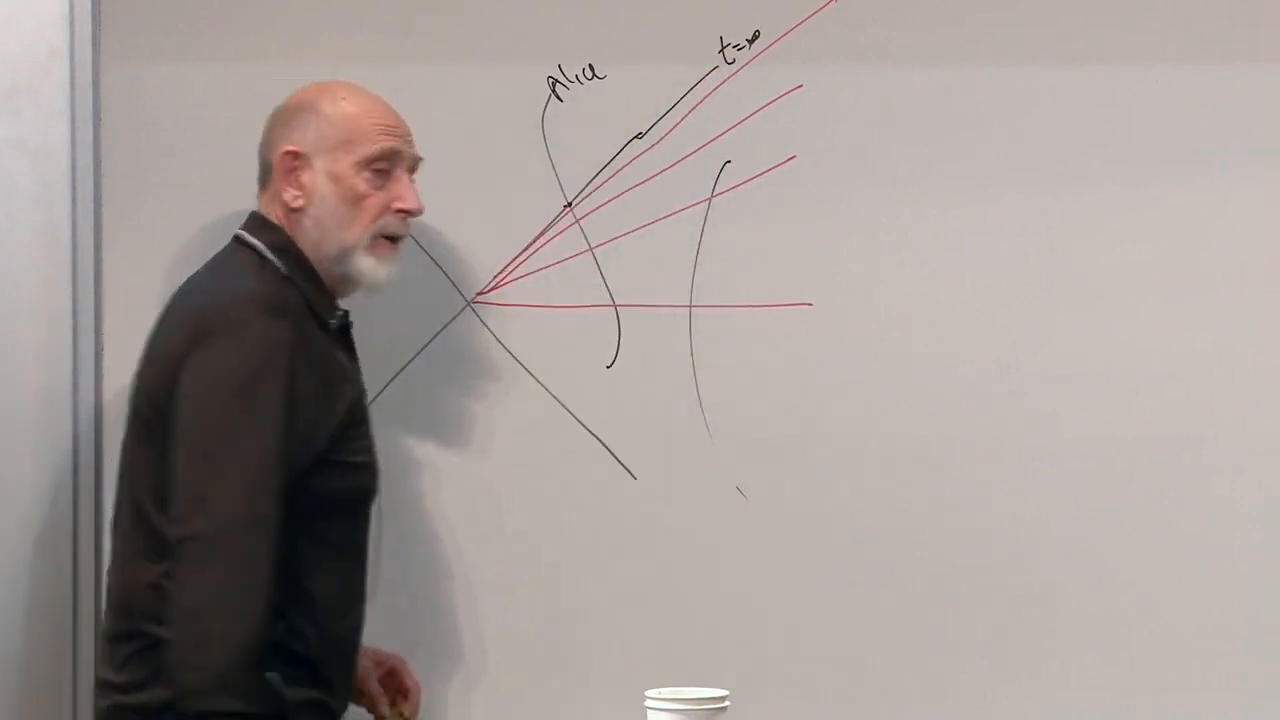
\includegraphics[width=0.84\textwidth]{lecture_07_figure_04.png}
\caption{La ligne d’univers d’Alice en chute et les demi-droites de temps de Schwarzschild constant. La demi-droite limite porte l’étiquette \(t=\infty\).}
\lectureframe{00:54:54}
\end{figure}

Alice est en chute libre. Sa ligne d’univers traverse l’horizon et atteint la singularité en un temps propre fini. Si le trou noir est assez grand pour que les forces de marée y soient faibles, rien de singulier n’arrive à son horloge à l’horizon.

Bob, lui, reste à rayon extérieur constant. Pour maintenir cette position, il doit accélérer. Les signaux lumineux émis à des instants de plus en plus tardifs sur la trajectoire d’Alice lui parviennent avec un retard croissant et un décalage vers le rouge de plus en plus prononcé. En temps de Schwarzschild, Alice s’approche de \(t=\infty\), et Bob ne reçoit jamais de signal émis après la traversée de son horizon. Ce sont des affirmations sur les signaux causaux et sur le feuilletage extérieur, et non des indices de l’existence d’une surface matérielle à l’horizon.

\begin{classroomqa}
\audiencequestion{Si Bob voit Alice ralentir, Alice doit-elle voir Bob accélérer ?}
\lecturerresponse{Non. Alice continue de recevoir des signaux lumineux ordinaires de Bob tant que sa ligne d’univers dure. Il existe un dernier événement sur la ligne d’univers de Bob qui peut lui parvenir, mais cet événement n’est le dernier que parce qu’Alice atteint ensuite la singularité. Rien n’arrive brusquement à Bob. Toute observation porte sur un cône de lumière passé, et les deux lignes d’univers entretiennent une relation causale asymétrique.
\lecturetimestamp{00:58:31--01:01:23}}
\end{classroomqa}

\begin{classroomqa}
\audiencequestion{Si Bob sait que, dans ses coordonnées, Alice est encore près de l’horizon, peut-il descendre, la récupérer et revenir ?}
\lecturerresponse{Une ligne d’univers de sauvetage doit rejoindre Alice avant qu’elle traverse l’horizon des événements. Après cet événement, aucun trajet futur ne peut la rejoindre puis revenir à l’extérieur. Le fait que les tranches de Schwarzschild situent la traversée en \(t=\infty\) ne signifie pas qu’Alice reste assise sur une surface matérielle où l’on pourrait la récupérer ; cela montre que ces tranches ne fournissent pas de notion globale de « maintenant » à travers l’horizon.
\lecturetimestamp{01:01:24--01:02:12}}
\end{classroomqa}

\section{Charlie suit Alice}

Faisons tomber Charlie à peu de distance derrière Alice. Tous deux sont alors approximativement inertiels près de l’horizon. Ils peuvent échanger des signaux, converser dans les deux sens ou même se tenir la main. Aucun des deux ne voit de panneau indiquant l’horizon. La différence avec Bob ne tient pas à l’identité des trois personnes, mais à celle entre la chute libre et une ligne d’univers accélérée qui reste à l’extérieur.

\begin{classroomqa}
\audiencequestion{Que voit Bob si Alice tombe la première et que Charlie la suit, comme un ballon de basket qui suit un anneau ?}
\lecturerresponse{Bob voit tous deux s’approcher de l’horizon. Alice, qui est devant, lui paraît ralentir progressivement et se comprimer radialement la première. Charlie semble se rapprocher de plus en plus d’elle, mais ne la rattrape jamais dans la vue limite de Bob depuis l’extérieur. Cette accumulation apparente ne décrit pas ce que ressent l’un ou l’autre des deux objets en chute.
\lecturetimestamp{01:04:12--01:06:05}}
\end{classroomqa}

\begin{classroomqa}
\audiencequestion{L’aplatissement apparent contredit-il la force de marée, qui devrait étirer l’objet en chute dans la direction radiale ?}
\lecturerresponse{Ce sont des effets différents. L’aplatissement relève de la description de Bob en coordonnées de Schwarzschild. L’allongement de marée est un effet local de la courbure que ressentent Alice et Charlie. La discussion suppose que le trou noir est assez grand, ou les observateurs assez petits, pour que l’effet de marée à l’horizon soit négligeable. Un trou noir d’environ une masse solaire produirait au contraire de fortes marées à l’horizon, tandis qu’elles peuvent être faibles pour un trou noir supermassif.
\lecturetimestamp{01:06:07--01:08:18}}
\end{classroomqa}

\begin{classroomqa}
\audiencequestion{Charlie voit-il Alice traverser l’horizon alors qu’il est encore à l’extérieur ?}
\lecturerresponse{Traçons le rayon nul. La lumière émise lors de la traversée d’Alice suit l’horizon et atteint Charlie au moment où celui-ci le traverse. À cet événement, il peut calculer qu’il a vu Alice traverser, même si aucun des deux observateurs ne rencontre de marqueur local. Ensuite, il peut la voir à l’intérieur. S’il accélère pour s’éloigner avant la traversée et parvient à rester à l’extérieur, il ne voit jamais la traversée.
\lecturetimestamp{01:08:19--01:11:11}}
\end{classroomqa}

\begin{classroomqa}
\audiencequestion{Si Alice est déjà à l’intérieur tandis que Charlie est à l’extérieur, comment comparer leurs rayons ultérieurs et leurs instants de traversée ?}
\lecturerresponse{Il n’existe pas de relation de simultanéité indépendante de l’observateur que l’on puisse déduire d’une expression comme « au même instant ». Alice voit Charlie sur son cône de lumière passé et ne peut voir sa traversée ultérieure que lorsqu’elle se trouve plus loin à l’intérieur. Ce sont les lignes d’univers et les rayons nuls précis qui répondent à la question. Pour généraliser à de nombreux objets en chute largement séparés, il faut tracer leur diagramme causal réel, au lieu de supposer un instant de traversée universel.
\lecturetimestamp{01:11:14--01:12:31}}
\end{classroomqa}

Dans les coordonnées régulières du voisinage de l’horizon, une trajectoire de chute libre est presque une droite. Elle n’est pas exactement rectiligne dans la géométrie complète de Schwarzschild, mais cette approximation devient bonne près d’un horizon vaste et faiblement courbé.

\begin{classroomqa}
\audiencequestion{La théorie des cordes peut-elle déterminer ce qui se passe dans le régime de gravité quantique à l’intérieur du trou noir ?}
\lecturerresponse{C’est précisément là que le sujet devient subtil. Une théorie quantique de la gravité est nécessaire près de la singularité, et la théorie des cordes est une candidate possible, mais les questions pertinentes étaient encore ouvertes et difficiles ; une simple application du diagramme classique ne les avait pas résolues.
\lecturetimestamp{01:13:04--01:13:38}}
\end{classroomqa}

\begin{classroomqa}
\audiencequestion{Que deviennent l’horloge et la vitesse propres d’Alice lorsqu’elle traverse l’horizon ?}
\lecturerresponse{Son horloge continue de battre à son rythme local ordinaire et mesure un temps propre fini. Dans son référentiel instantané de repos, elle est au repos ; relativement à un référentiel local en chute libre, sa vitesse est finie et ordinaire. Près d’un horizon vaste, la géométrie est presque plate, si bien que les marques régulièrement espacées en temps propre sur sa ligne d’univers restent régulières jusqu’à ce que la courbure devienne forte près de la singularité.
\lecturetimestamp{01:13:39--01:14:44}}
\end{classroomqa}

\begin{classroomqa}
\audiencequestion{Que se passe-t-il si Bob accélère vers l’extérieur, mais pas assez pour éviter de tomber à travers l’horizon ?}
\lecturerresponse{Sa ligne d’univers se courbe alors vers l’extérieur, mais traverse tout de même l’horizon. S’il le traverse très tard, il peut voir Alice peu après sa propre traversée, mais le temps propre qui lui reste avant la singularité est court. Les pentes des lignes d’univers sur le croquis ne sont pas des étalons ni des horloges gradués ; c’est l’ordre causal, et non leurs longueurs euclidiennes dessinées, qui est préservé.
\lecturetimestamp{01:14:47--01:16:31}}
\end{classroomqa}

Toutes ces conclusions supposent qu’aucun signal ne dépasse la vitesse de la lumière. Le cours plaisante brièvement au sujet de reportages de presse récents à l’époque, qui évoquaient des neutrinos apparemment supraluminiques en Italie ; il s’agissait d’une allusion à une erreur de chronométrage expérimental, et non d’une exception à la relativité. La construction causale elle-même reste bornée par les droites nulles.

\begin{classroomqa}
\audiencequestion{Des horloges synchronisées portées par Alice et Bob peuvent-elles trancher la question si Alice plonge vers l’horizon puis revient ?}
\lecturerresponse{Ils peuvent comparer leurs horloges lorsqu’ils se retrouvent au même endroit, mais après la séparation de leurs lignes d’univers, il n’existe pas de synchronisation distante unique, surtout lorsque l’un d’eux change de mouvement. Traçons les deux lignes d’univers et les rayons nuls échangés. Ce diagramme donne la réponse opérationnelle à toute expérience spécifiée.
\lecturetimestamp{01:17:34--01:18:25}}
\end{classroomqa}

\begin{figure}[htbp]
\centering
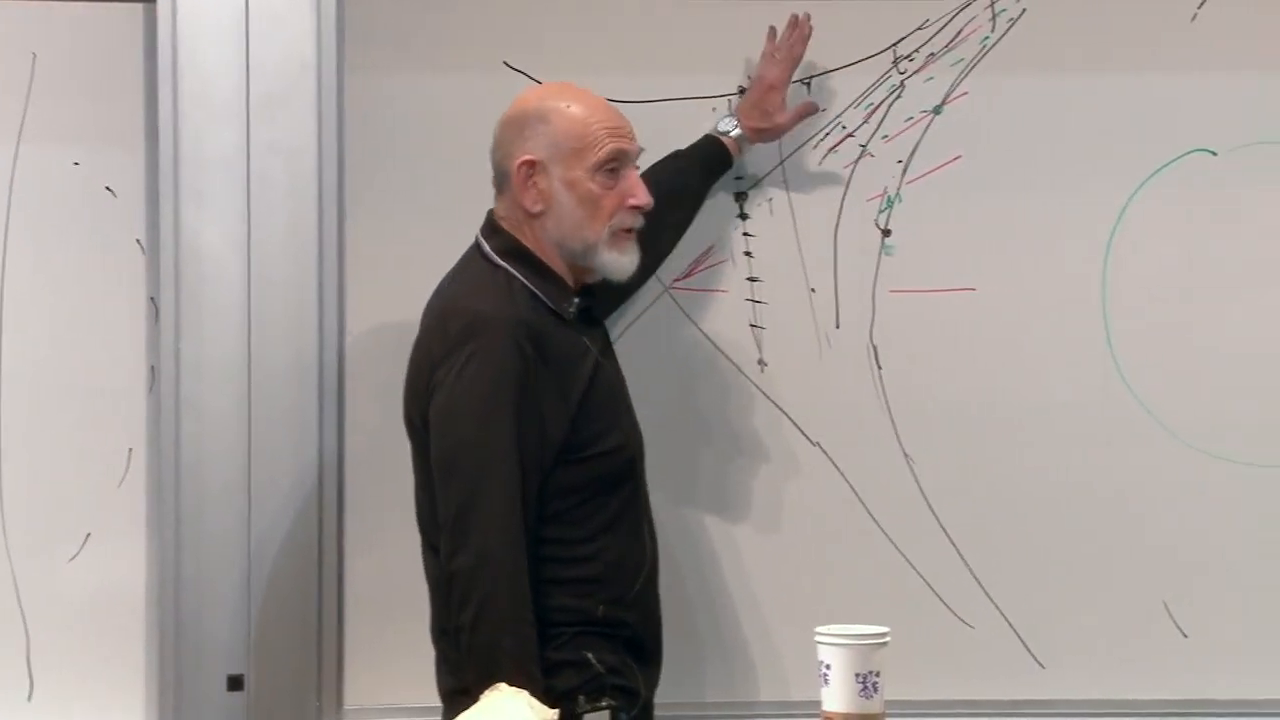
\includegraphics[width=0.86\textwidth]{lecture_07_figure_05.png}
\caption{Le diagramme causal construit progressivement pour répondre aux questions sur Alice, Bob et Charlie. Chaque observation se situe en traçant un rayon nul depuis l’événement observé jusqu’à la ligne d’univers de l’observateur.}
\lectureframe{01:18:12}
\end{figure}

\begin{figure}[htbp]
\centering
\resizebox{0.96\linewidth}{!}{%
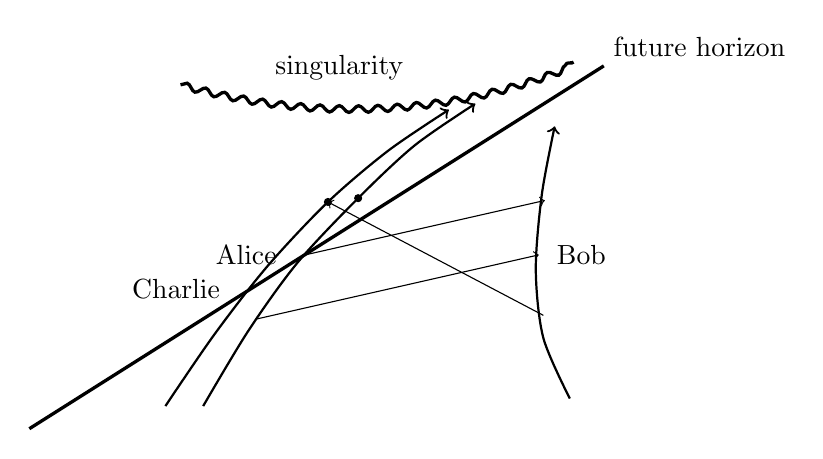
\begin{tikzpicture}[scale=0.96]
\draw[very thick] (-3.8,-0.3) -- (3.8,4.5);
\node[above right] at (3.8,4.5) {future horizon};
\draw[very thick,decorate,decoration={snake,amplitude=1.2pt,segment length=7pt}]
  (-1.8,4.25) .. controls (0.1,3.72) and (2.0,3.92) .. (3.4,4.55);
\node at (0.3,4.48) {singularity};
\draw[thick,->]
  plot[smooth] coordinates {(-1.5,0.0) (-0.9,1.0) (-0.25,1.9)
  (0.55,2.75) (1.3,3.45) (2.1,4.0)};
\node[left] at (-0.4,2.0) {Alice};
\draw[thick,->]
  plot[smooth] coordinates {(-2.0,0.0) (-1.35,0.95) (-0.65,1.85)
  (0.15,2.7) (0.95,3.38) (1.75,3.92)};
\node[left] at (-1.15,1.55) {Charlie};
\draw[thick,->]
  plot[smooth] coordinates {(3.35,0.1) (3.0,0.9) (2.9,1.8)
  (2.98,2.8) (3.15,3.7)};
\node[right] at (3.05,2.0) {Bob};
\draw[thin,->] (-0.8,1.15) -- (2.94,2.0);
\draw[thin,->] (-0.15,2.0) -- (3.02,2.72);
\draw[thin,->] (3.0,1.2) -- (0.15,2.7);
\draw[fill] (0.55,2.75) circle (1.3pt);
\draw[fill] (0.15,2.7) circle (1.3pt);
\end{tikzpicture}
}
\caption{Schéma des observateurs. Les observations de Bob depuis l’extérieur et les observations mutuelles d’Alice et Charlie reposent sur des constructions distinctes de rayons nuls, et non sur des slogans de réciprocité entre horloges.}
\label{fig:l7-observers-clean}
\end{figure}

\begin{classroomqa}
\audiencequestion{Bob voit-il Alice pendant un temps infini, et cela signifie-t-il qu’elle ne meurt jamais dans sa réalité ?}
\lecturerresponse{Bob reçoit ses signaux pendant un intervalle de son temps qui n’est pas borné, mais il voit son horloge ralentir jusqu’à un rythme nul et ne reçoit que la suite finie de battements de cœur émis avant sa traversée. Le mot « réalité » masque la distinction entre un événement local et le relevé asymptotique d’un observateur. Alice ne voit pas son horloge s’arrêter à l’horizon ; les signaux reçus par Bob sont de plus en plus retardés et décalés vers le rouge.
\lecturetimestamp{01:18:32--01:20:59}}
\end{classroomqa}

\begin{classroomqa}
\audiencequestion{Une fois qu’Alice a traversé l’horizon, voit-elle soudain toute la matière ancienne qui paraissait figée à celui-ci ?}
\lecturerresponse{Rien ne se dégage brusquement. Pendant sa chute, les cônes de lumière passés qui lui permettent de voir la matière antérieure changent continûment. Elle peut déduire que la lumière qui lui parvient maintenant a été émise plus tôt et que la matière a traversé l’horizon avant elle. Le point de vue de Charlie sur Alice enseigne la même chose : aucune des traversées ne produit de discontinuité locale ni ne révèle un amas caché de chaises et de dinosaures.
\lecturetimestamp{01:21:02--01:23:48}}
\end{classroomqa}

\begin{classroomqa}
\audiencequestion{Existe-t-il des simulations réalistes de ce qu’un objet en chute verrait ?}
\lecturerresponse{Le cours renvoie aux visualisations de trous noirs d’Andrew Hamilton. Elles peuvent rendre perceptibles l’aberration marquée et les décalages de fréquence de la lumière entrante, même si l’image peut déconcerter davantage qu’éclairer. L’expression « rien de particulier à l’horizon » concerne la géométrie locale, et non l’apparence ordinaire du ciel.
\lecturetimestamp{01:24:11--01:25:29}}
\end{classroomqa}

\section{D’un trou éternel à un trou en croissance}

Le sommet inférieur du diagramme éternel maximalement prolongé a peu de signification directe pour un trou noir formé par l’effondrement d’une étoile. Dans la géométrie simple de l’effondrement, seule apparaît la partie contenant l’extérieur, l’horizon futur et l’intérieur futur. Cette distinction devient essentielle lorsque la matière peut faire varier la masse du trou noir.

\begin{classroomqa}
\audiencequestion{Quel événement physique représente le sommet inférieur du diagramme idéalisé ?}
\lecturerresponse{Dans la solution mathématique éternelle, il fait partie du prolongement maximal. Un trou noir formé par l’effondrement de matière ne contient pas toute cette région inférieure. Son horizon a une histoire de formation, qui exige un autre diagramme global et sera étudiée au cours suivant.
\lecturetimestamp{01:25:59--01:26:52}}
\end{classroomqa}

Lorsqu’un petit corps d’épreuve tombe dans le trou noir, on peut négliger sa rétroaction et le diagramme de Schwarzschild fixe suffit. Si une masse importante tombe dans le trou noir, la masse de celui-ci et le rayon de Schwarzschild augmentent :
\begin{equation}
r_{\mathrm S}=2GM,
\qquad
\Delta r_{\mathrm S}=2G\,\Delta M.
\label{eq:l7-growing-radius}
\end{equation}
L’horizon se déforme vers l’objet entrant, les horizons se rejoignent et l’horizon commun déformé se stabilise rapidement. Dans l’idéalisation non rotative du cours, l’état final est une sphère légèrement plus grande. Une fusion réelle rayonne aussi de l’énergie sous forme d’ondes gravitationnelles et laisse généralement un trou noir en rotation.

\begin{classroomqa}
\audiencequestion{Si l’horizon grandit lorsqu’une masse tombe dans le trou noir, se déplace-t-il vers l’extérieur pour rejoindre la matière qui semblait figée près de l’ancien horizon ?}
\lecturerresponse{Pour un objet entrant suffisamment massif, l’approximation de la particule d’épreuve n’est plus valable. L’horizon se déforme, rejoint la région piégée de l’objet entrant et se détend vers un horizon stationnaire plus grand. La position exacte de l’horizon des événements est de nature globale et peut s’étendre dans une région antérieure à l’arrivée de la matière. Le cours reporte délibérément la construction complète à la prochaine séance.
\lecturetimestamp{01:26:55--01:29:05}}
\end{classroomqa}

\begin{classroomqa}
\audiencequestion{Pourquoi les astronomes peuvent-ils observer des éclats lumineux si la matière met un temps de Schwarzschild infini à atteindre l’horizon ?}
\lecturerresponse{Le rayonnement lumineux intense ne provient pas de l’horizon lui-même. Dans un flux ou un disque d’accrétion, le gaz entre en collision et s’échauffe à l’extérieur de l’horizon, notamment près des orbites photoniques fortement courbées. Ce plasma extérieur peut émettre de la lumière qui nous parvient. La géométrie vide de Schwarzschild isole le problème causal, mais ne constitue pas un modèle complet d’un environnement astrophysique.
\lecturetimestamp{01:29:07--01:30:22}}
\end{classroomqa}

Le temps caractéristique de relaxation est fixé par le temps de traversée de la lumière :
\begin{equation}
t_{\mathrm{cross}}\sim\frac{r_{\mathrm S}}{c},
\qquad
t_{\mathrm{relax}}\sim
\text{a few to a few tens of }t_{\mathrm{cross}}.
\label{eq:l7-relaxation-scale}
\end{equation}
Le cours estime que \(10^{-5}\,\mathrm{s}\) correspond au temps de traversée d’un trou noir de l’ordre du kilomètre et qu’il faut environ \(10^{-3}\,\mathrm{s}\) pour qu’une petite fusion devienne presque stationnaire. Pour un trou noir d’un milliard de masses solaires, le temps correspondant se compte en minutes ou en heures. Ce sont des estimations d’échelle, et non des calculs précis de fusion. C’est la succession géométrique qui importe : haltère, cacahuète, presque sphérique, stationnaire.

\begin{classroomqa}
\audiencequestion{À quelle vitesse un horizon déformé ou issu d’une fusion récente se stabilise-t-il ?}
\lecturerresponse{Sur une échelle de temps qui ne dépasse pas de beaucoup le temps nécessaire à la lumière pour traverser le trou noir. Comme toutes les longueurs et tous les temps varient avec \(r_{\mathrm S}\), les petits trous noirs se stabilisent en une fraction de seconde, tandis que les trous supermassifs le font selon des temps d’horloge beaucoup plus longs. L’absence de cheveux décrit l’état final stationnaire ; la déformation transitoire évacue de l’énergie sous forme de rayonnement gravitationnel.
\lecturetimestamp{01:30:26--01:33:18}}
\end{classroomqa}

\begin{classroomqa}
\audiencequestion{Que voit Bob si de la matière tombée plus tôt se trouve entre l’ancien et le nouvel horizon tandis qu’un autre corps massif tombe dans le trou noir ?}
\lecturerresponse{Il est impossible de répondre de manière cohérente à cette question en raccordant deux diagrammes statiques de Schwarzschild. Il faut résoudre ou construire la géométrie d’effondrement dépendante du temps et déterminer la position de son horizon global. Le cours laisse la question en suspens et reporte explicitement la réponse à la semaine suivante, consacrée à la formation des horizons.
\lecturetimestamp{01:33:20--01:35:41}}
\end{classroomqa}

\section{Que change la variation d’échelle ?}

Le diagramme sans dimension ne change pas lorsque \(r_{\mathrm S}\) varie. En revanche, la signification physique d’un intervalle dessiné change :
\begin{equation}
d\tau_{\mathrm{physical}}^2
=
r_{\mathrm S}^2\,d\hat{\tau}^2,
\qquad
\ell_{\mathrm{physical}}
=
r_{\mathrm S}\,\hat{\ell}.
\label{eq:l7-scale-restoration}
\end{equation}
Une séparation sans dimension qui représente un demi-kilomètre pour un trou noir de l’ordre du kilomètre en représente environ un demi-milliard de kilomètres pour un trou noir mille millions de fois plus grand. L’analogie des sphères dessinées à la même taille revient ici : la forme reste la même, tandis que le nombre de mètres étalons représenté par une ligne varie avec le rayon.

\begin{classroomqa}
\audiencequestion{Comment le diagramme causal change-t-il lorsque le rayon de Schwarzschild varie ?}
\lecturerresponse{Il ne change pas une fois le rayon éliminé par changement d’échelle. Chaque longueur et chaque durée physique attribuée au diagramme est multipliée par \(r_{\mathrm S}\), tandis que la courbure aux points sans dimension correspondants est multipliée par \(r_{\mathrm S}^{-2}\).
\lecturetimestamp{01:35:41--01:38:10}}
\end{classroomqa}

\begin{classroomqa}
\audiencequestion{La conclusion causale change-t-elle si Bob est en orbite plutôt que de rester à une position angulaire fixe ?}
\lecturerresponse{Les décalages vers le rouge détaillés et les directions d’arrivée deviennent plus complexes, mais la séparation causale due à l’horizon ne change pas. Aucune orbite temporelle extérieure ne reçoit de signal émis depuis l’intérieur de l’horizon.
\lecturetimestamp{01:38:12--01:38:26}}
\end{classroomqa}

\begin{classroomqa}
\audiencequestion{Puisque la gravité s’annule à l’intérieur d’une coquille sphérique, s’annule-t-elle aussi à l’intérieur de l’horizon parce que la masse du trou noir est répartie sur cette surface ?}
\lecturerresponse{Non. L’horizon des événements n’est pas une coquille matérielle qui porterait la masse. Le théorème newtonien des coquilles ne s’y applique donc pas. Le cours compare la solution statique extérieure à une source ponctuelle située à la singularité de courbure, mais la matière qui tombe actuellement au cours de la formation du trou noir exige la géométrie dépendant du temps, qui sera étudiée au cours suivant.
\lecturetimestamp{01:38:28--01:40:41}}
\end{classroomqa}

\section{Rotation et géométrie radiale}

Le moment cinétique subsiste après l’effondrement. La géométrie extérieure d’un trou noir en rotation diffère de celle de Schwarzschild : sa solution stationnaire est celle de Kerr, la rotation déforme la géométrie de l’horizon et l’entraînement des référentiels fait tourner les directions inertielles autour du trou. En principe, on mesure le moment cinétique à partir de ces effets gravitationnels extérieurs. La matière ne perd pas son moment cinétique simplement en franchissant un horizon.

\begin{classroomqa}
\audiencequestion{Un trou noir peut-il avoir un moment cinétique mesurable, et la rotation modifie-t-elle la gravité à l’extérieur ?}
\lecturerresponse{Oui. Le moment cinétique subsiste comme paramètre conservé, déforme la géométrie stationnaire et produit un entraînement des référentiels. L’horizon n’est plus le simple horizon sphérique de Schwarzschild. Le cours compare qualitativement cette déformation à la forme aplatie de la Terre, tout en soulignant que la solution complète en rotation est nettement plus complexe.
\lecturetimestamp{01:40:45--01:42:36}}
\end{classroomqa}

\begin{classroomqa}
\audiencequestion{La relation entre \(r\) et la distance propre \(\rho\) signifie-t-elle que la gravité contracte l’espace ?}
\lecturerresponse{La distance radiale propre \(\rho\) vérifie
\begin{equation*}
\frac{d\rho}{dr}=\sqrt{\frac{r}{r-1}}>1
\end{equation*}
À l’extérieur de l’horizon unité. Un accroissement coordonné donné \(dr\) correspond donc à un intervalle radial propre plus grand près de l’horizon. Dire que l’espace est contracté ou étiré dépend des intervalles de coordonnées que l’on compare. L’énoncé invariant est la relation entre les distances propres elle-même.
\lecturetimestamp{01:42:36--01:43:20}}
\end{classroomqa}

\section{Questions finales}

\begin{classroomqa}
\audiencequestion{Du point de vue de Bob, l’horloge d’Alice semble s’arrêter. Du point de vue d’Alice, l’espace ou le temps de Bob prend-il fin ?}
\lecturerresponse{Non. Alice voit les signaux ordinaires provenant d’événements successifs sur la ligne d’univers de Bob, jusqu’à ce que sa propre ligne d’univers prenne fin. Elle ne voit pas les événements ultérieurs de Bob parce qu’aucun point ultérieur n’existe sur sa ligne d’univers, et non parce que Bob ou son espace disparaît. Dans ces coordonnées causales régulières, les rayons lumineux radiaux sont représentés par des lignes droites ; leur apparence de trajectoires courbes dans un autre système de coordonnées ne change pas les événements qu’ils relient.
\lecturetimestamp{01:43:21--01:45:20}}
\end{classroomqa}

La relativité générale comporte deux tâches complémentaires. Étant donnée une métrique, on peut tracer les géodésiques et les rayons lumineux afin de déterminer ce que mesurent les observateurs. Étant donnée une distribution de matière, il faut résoudre les équations d’Einstein pour trouver la métrique. La première tâche a occupé ce cours. La seconde est généralement plus difficile, bien que l’effondrement avec symétrie fournisse des exemples traitables.

\begin{classroomqa}
\audiencequestion{Qu’advient-il de l’horizon et de la singularité d’un trou noir qui s’évapore ?}
\lecturerresponse{Le cours présente un schéma qualitatif dans lequel l’horizon se rétrécit et rejoint l’extrémité de la région singulière. L’évaporation est un processus quantique semi-classique, et le devenir final à l’échelle de Planck n’est pas déterminé par le diagramme classique de Schwarzschild. Il faut donc voir ce schéma de rétrécissement comme un aperçu qualitatif, et non comme une géométrie quantique complète.
\lecturetimestamp{01:46:04--01:46:32}}
\end{classroomqa}

Presque tous les trous noirs astrophysiques devraient être en rotation. Les étoiles possèdent déjà un moment cinétique, et l’effondrement amplifie leur vitesse angulaire à la manière bien connue d’un patineur qui ramène les bras vers lui. La structure singulière d’un trou noir de Kerr n’est pas la surface de Schwarzschild \(r=0\) représentée ici ; il ne faut pas la décrire comme de la matière tournant littéralement à une vitesse linéaire infinie.

\begin{classroomqa}
\audiencequestion{Les trous noirs macroscopiques sans rotation sont-ils courants, et combien y a-t-il de trous noirs ?}
\lecturerresponse{Un moment cinétique exactement nul serait une idéalisation exceptionnelle. Le cours ne donne qu’une estimation pédagogique très approximative de la population cosmique, comprise entre les nombres de galaxies et d’étoiles, et peut-être de l’ordre de \(10^{15}\). Il s’agit d’une estimation datant du cours, et non d’un recensement mesuré. Le point solide est que l’effondrement conserve et amplifie généralement une partie du moment cinétique.
\lecturetimestamp{01:46:32--01:48:42}}
\end{classroomqa}

\begin{classroomqa}
\audiencequestion{Les trous noirs se forment-ils à partir de matière préexistante ou apparaissent-ils par un processus quantique ?}
\lecturerresponse{Les trous noirs astrophysiques ordinaires se forment lorsque de la matière stellaire existante s’effondre. La combustion nucléaire et le flux d’énergie vers l’extérieur contribuent à soutenir une étoile. Lorsque son combustible est épuisé, le résidu se contracte. Selon sa masse et les mécanismes de soutien par la pression dont il dispose, il peut devenir une naine blanche ou une étoile à neutrons ; si aucun soutien ne peut arrêter l’effondrement, il peut aussi passer sous son propre rayon de Schwarzschild et former un trou noir.
\lecturetimestamp{01:48:43--01:50:23}}
\end{classroomqa}

\begin{classroomqa}
\audiencequestion{Des trous noirs microscopiques pourraient-ils se former, et qu’est-ce qui déterminerait leur durée de vie et leur taille minimale ?}
\lecturerresponse{Cette partie est spéculative. L’évaporation de Hawking est d’autant plus rapide que la masse est faible, et la durée de vie varie approximativement comme \(M^3\). Le cours compare un trou noir dont la durée de vie pourrait être cosmologique à une montagne en termes de masse ; cette analogie numérique n’est qu’approximative. Des fluctuations très fortes de densité dans l’Univers primordial ou des collisions suffisamment énergétiques pourraient constituer des mécanismes de formation. Un trou noir proche de la masse de Planck, soit environ \(10^{-5}\,\mathrm{g}\), marque l’échelle à laquelle une description géométrique classique cesse d’être fiable. Selon une extrapolation directe, atteindre cette énergie dans un accélérateur ordinaire exigerait une machine d’une taille invraisemblable, même si la formation est possible en principe.
\lecturetimestamp{01:50:23--01:53:31}}
\end{classroomqa}

\begin{classroomqa}
\audiencequestion{Le cours abordera-t-il la cosmologie, la matière noire, l’énergie noire, l’entropie et les ondes gravitationnelles ?}
\lecturerresponse{Les applications cosmologiques et, peut-être, les ondes gravitationnelles restent des sujets possibles pour la suite. L’entropie des trous noirs est reportée au-delà du trimestre. Le cours se conclut en reconnaissant que seulement environ un quart du programme prévu a été couvert ce soir-là : répondre soigneusement aux questions compte davantage que de parcourir le plan à toute vitesse.
\lecturetimestamp{01:53:33--01:54:38}}
\end{classroomqa}

La règle opérationnelle résiste à toutes les questions posées dans la salle. Précisez les lignes d’univers, tracez les rayons lumineux et repérez les événements qu’ils relient. L’horizon n’est pas un lieu où la physique locale cesse de fonctionner ; c’est la frontière au-delà de laquelle tout signal dirigé vers le futur reste à l’intérieur. Le cours suivant remplacera le fond éternel par une source en effondrement et montrera comment cette frontière se forme.